\chapter{Chapter I}
\section{Langkah-langkah Membuat Aplikasi Pada Oracle Apex Dengan Data Mahasiswa}

\begin{enumerate}
\item Login
    \begin{figure}[!htbp]
    \centering
    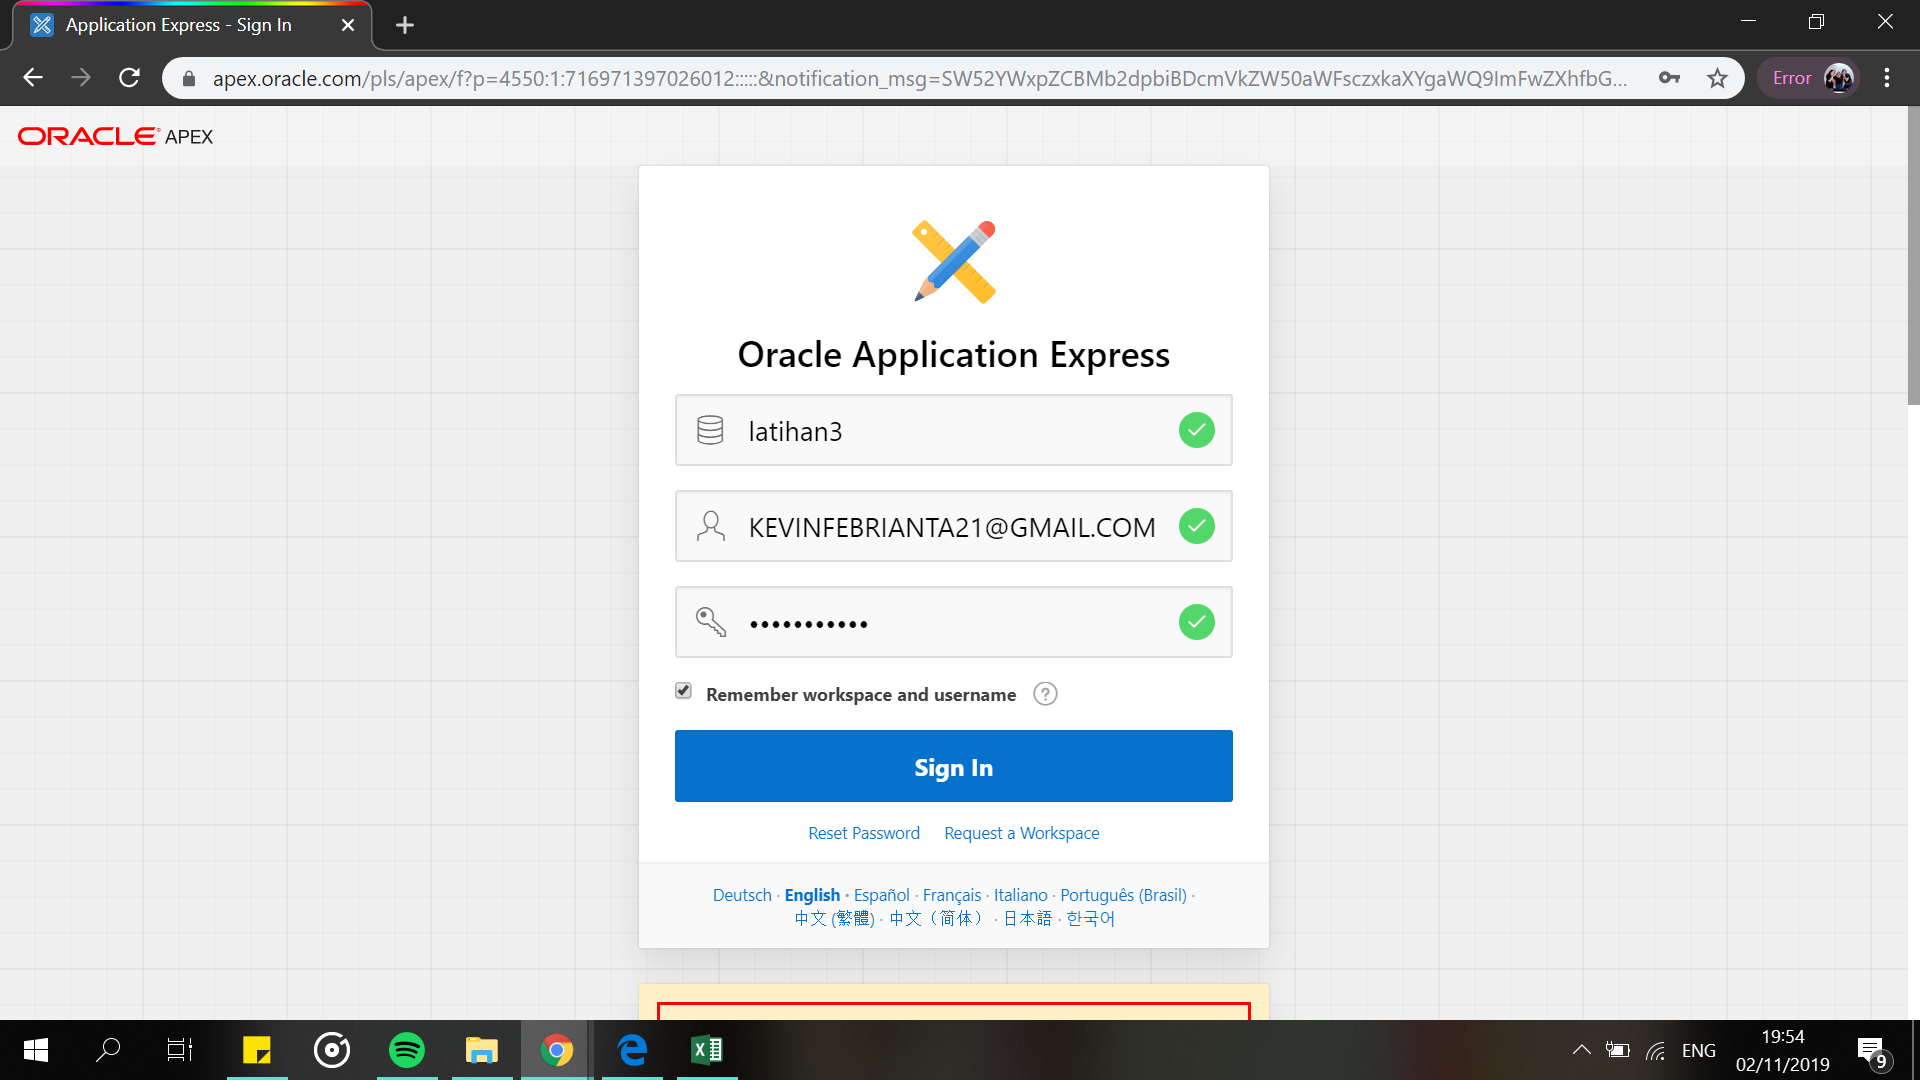
\includegraphics[width=9cm]{picture/01.png}
    \caption{Login}
    \end{figure}
    
\item Pilih app builder
    \begin{figure}[!htbp]
    \centering
    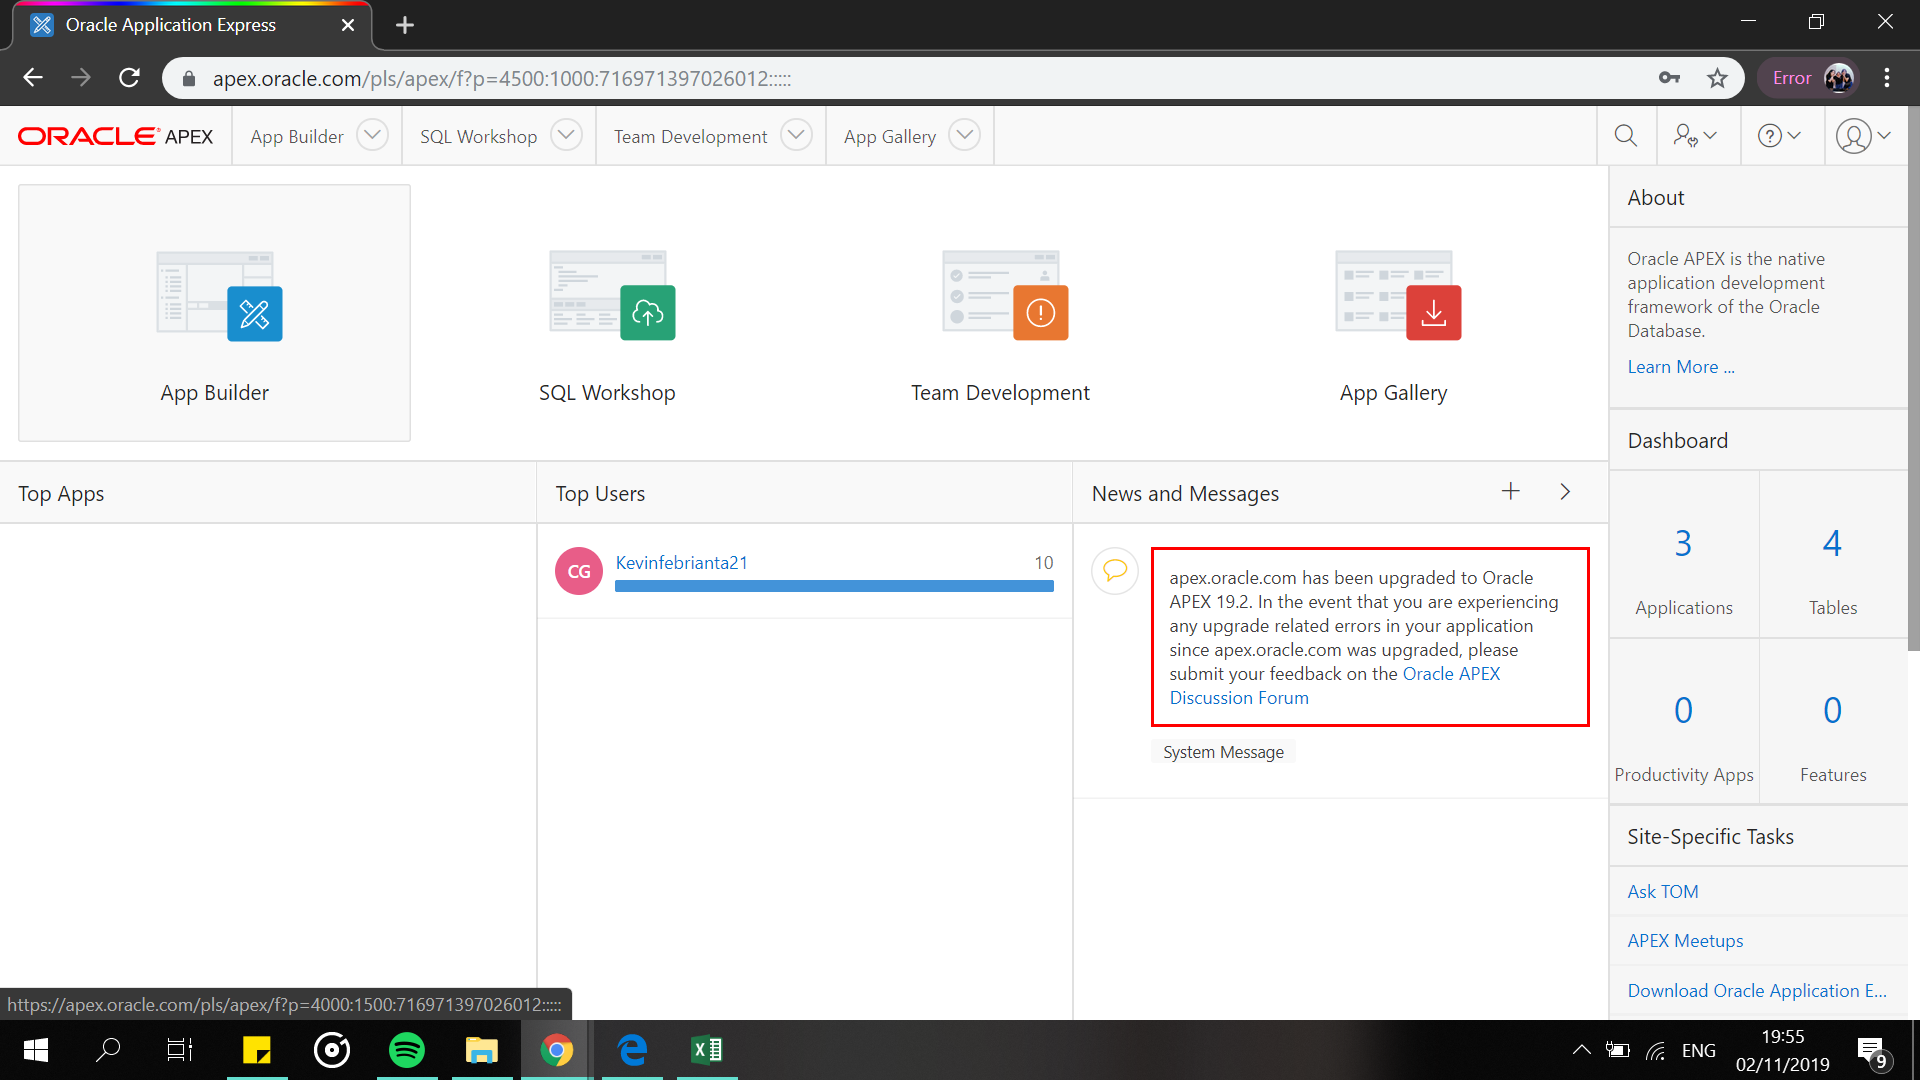
\includegraphics[width=9cm]{picture/02.png}
    \caption{Pilih App Builder}
    \end{figure}
    
\newpage
\item Untuk memasukkan data dari pc, kita pilih create.
    \begin{figure}[!htbp]
    \centering
    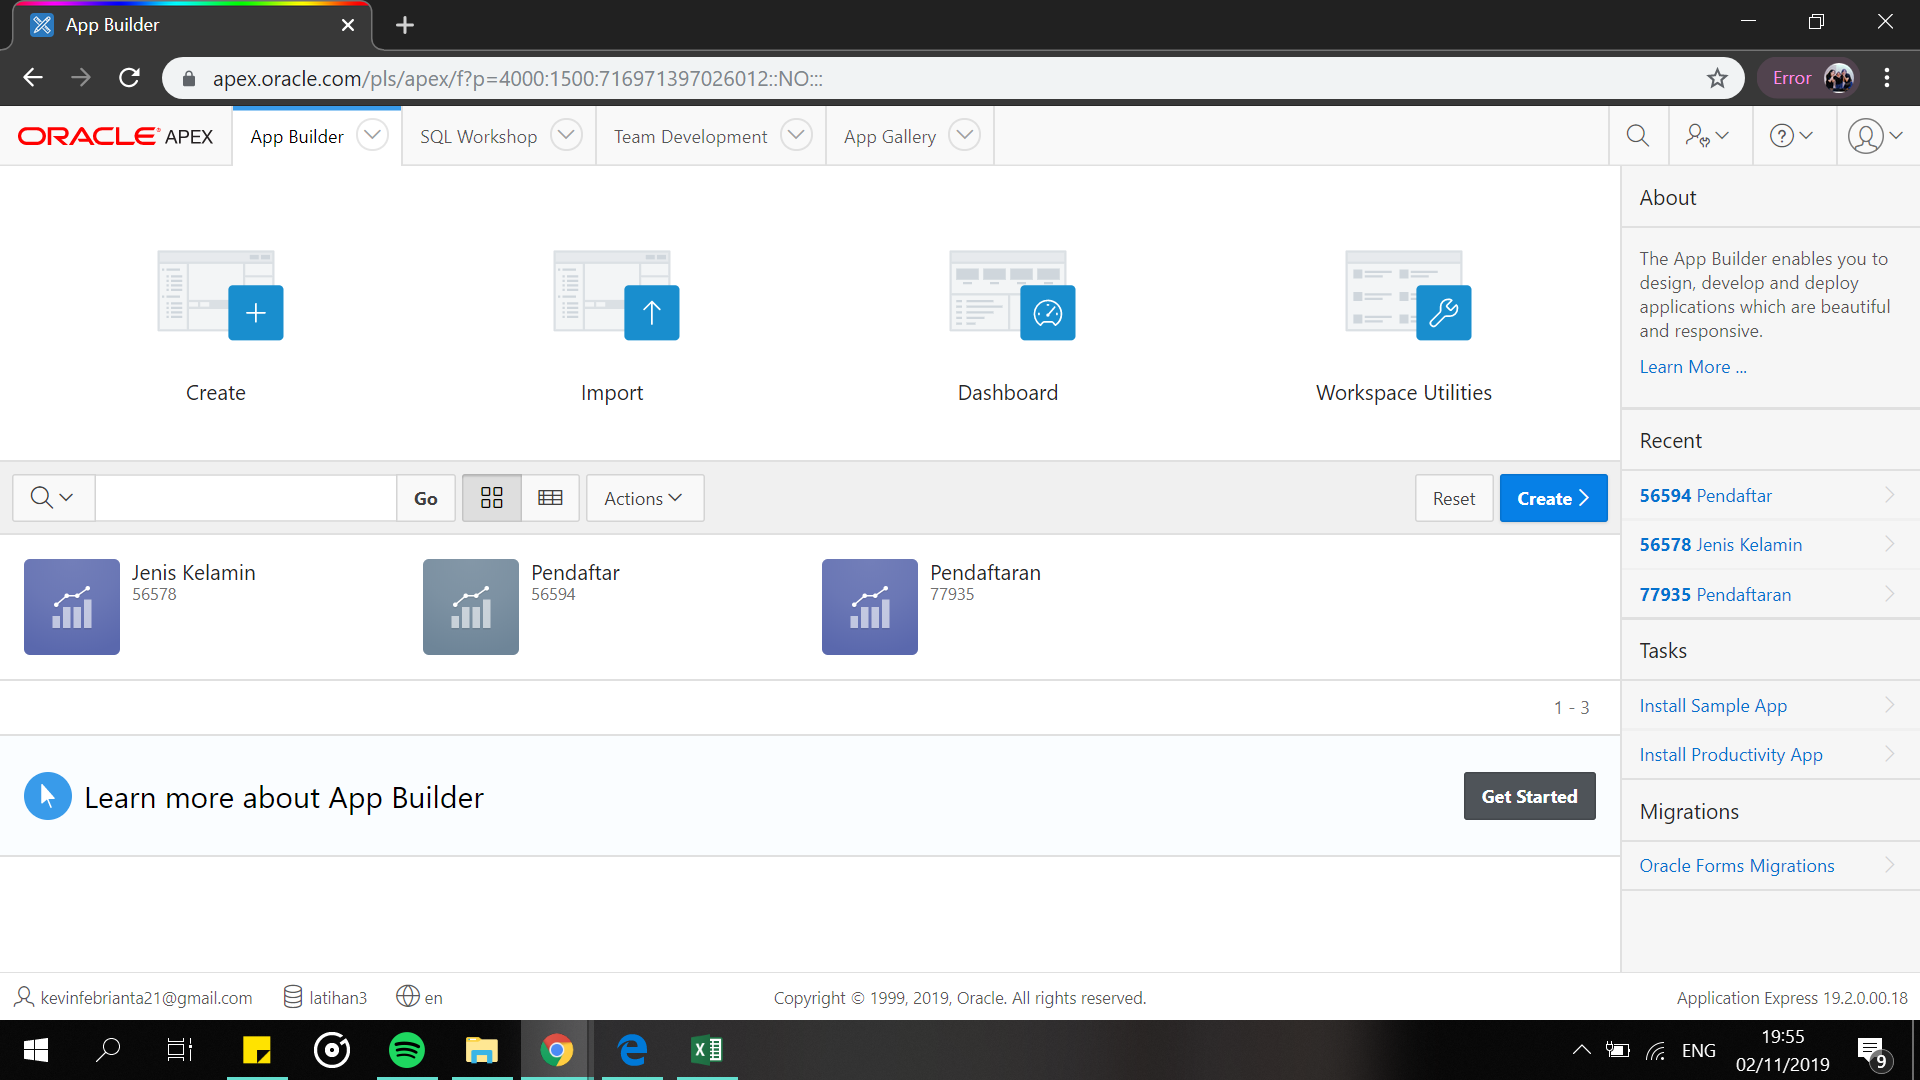
\includegraphics[width=8cm]{picture/03.png}
    \caption{Create}
    \end{figure}
    
\item  Untuk memasukkan data kita pilih From a file ,jika sudah kita pilih data mahasiswa yang ingin dimasukkan
    \begin{figure}[!htbp]
    \centering
    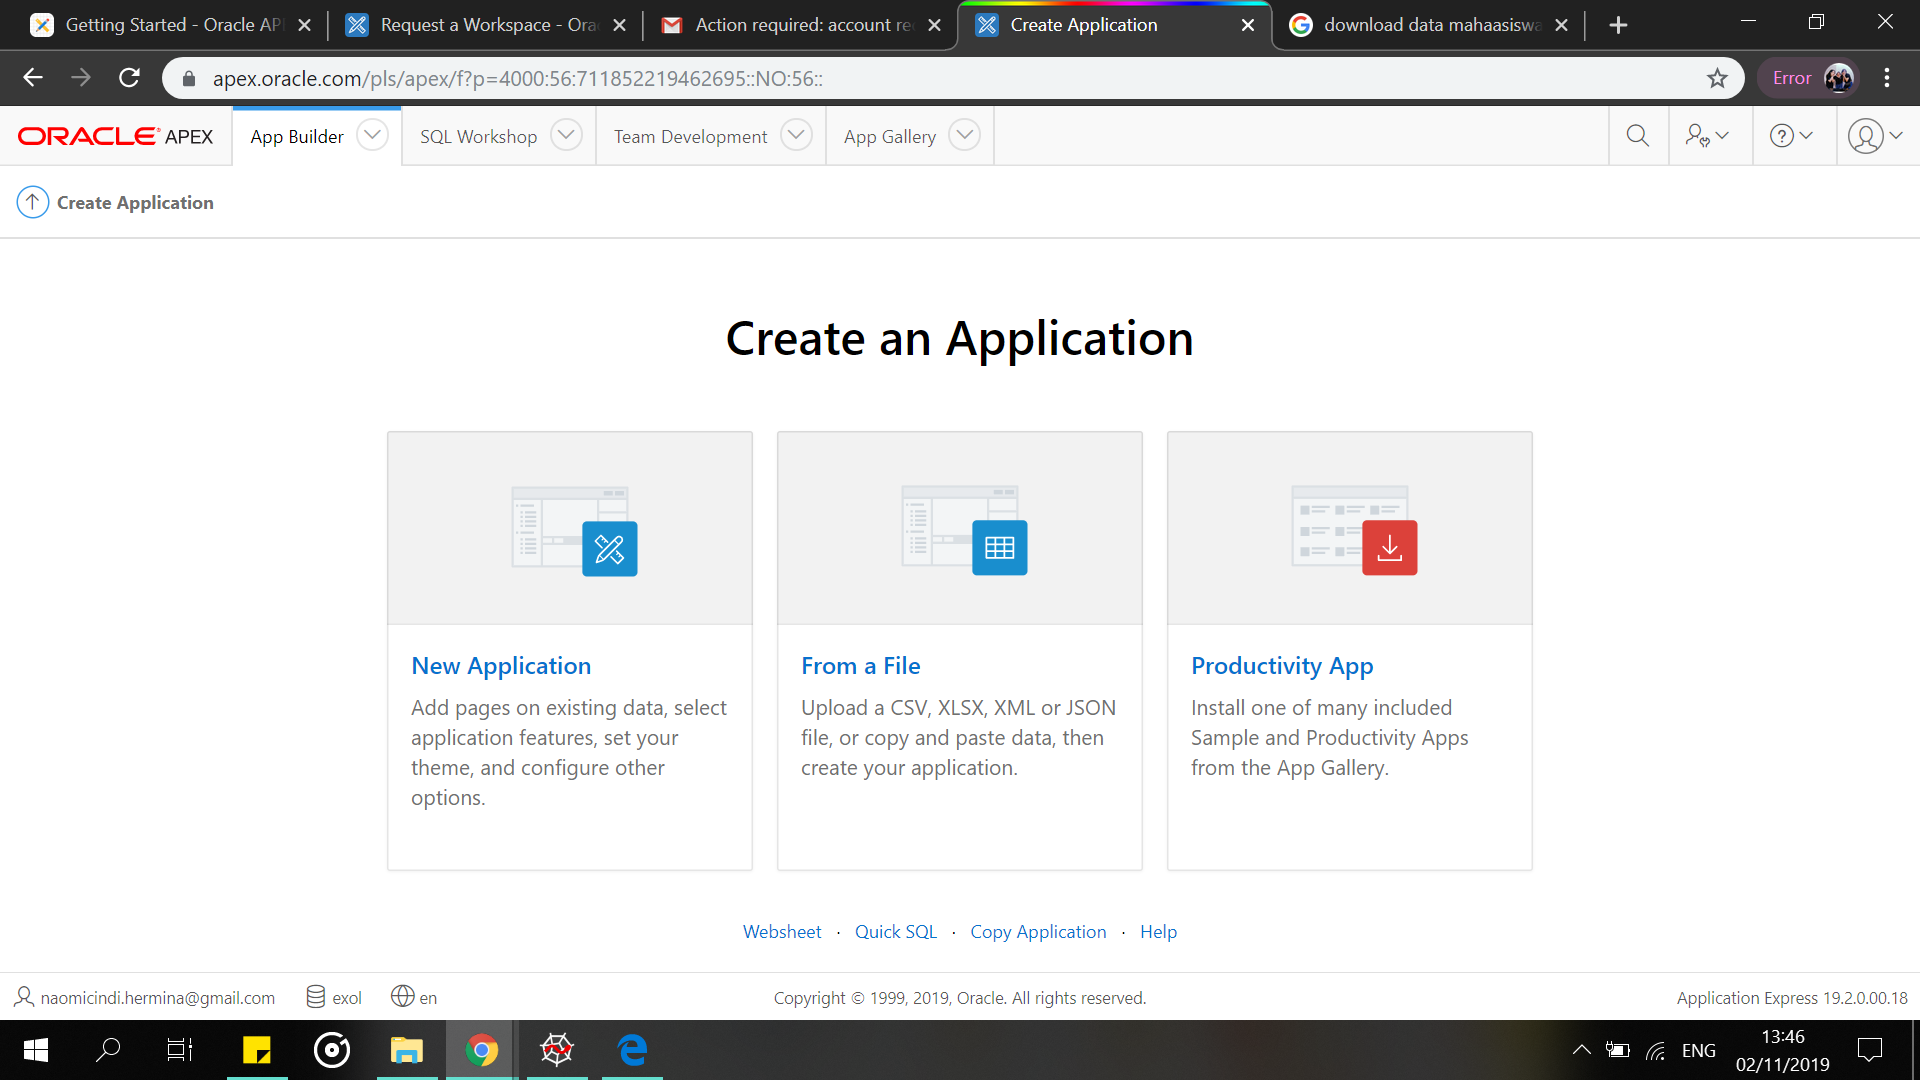
\includegraphics[width=8cm]{picture/09.png}
    \caption{Upload File}
    \end{figure}

\item Jika data telah berhasil di input maka akan muncul tampilan
    \begin{figure}[!htbp]
    \centering
    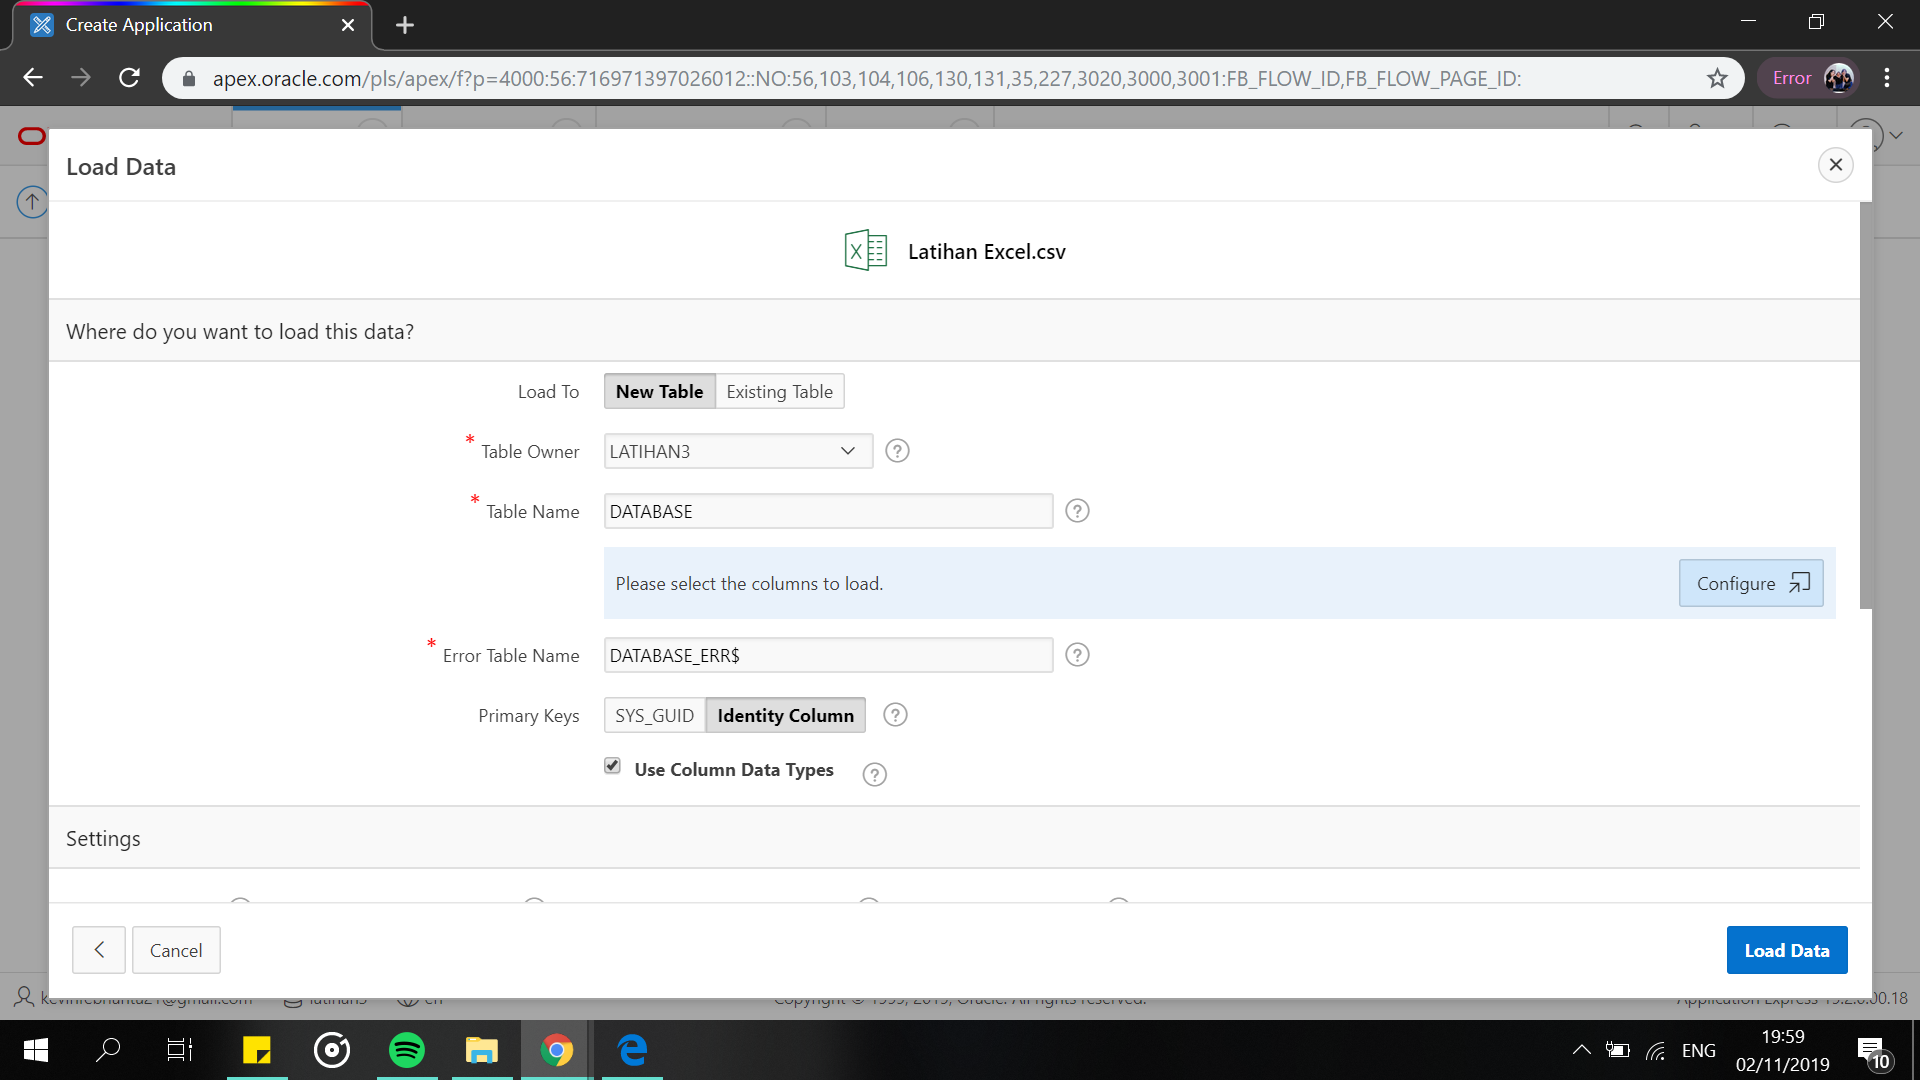
\includegraphics[width=8cm]{picture/04.png}
    \caption{Mengisi Nama Tabel}
    \end{figure}
    
    \begin{figure}[!htbp]
    \centering
    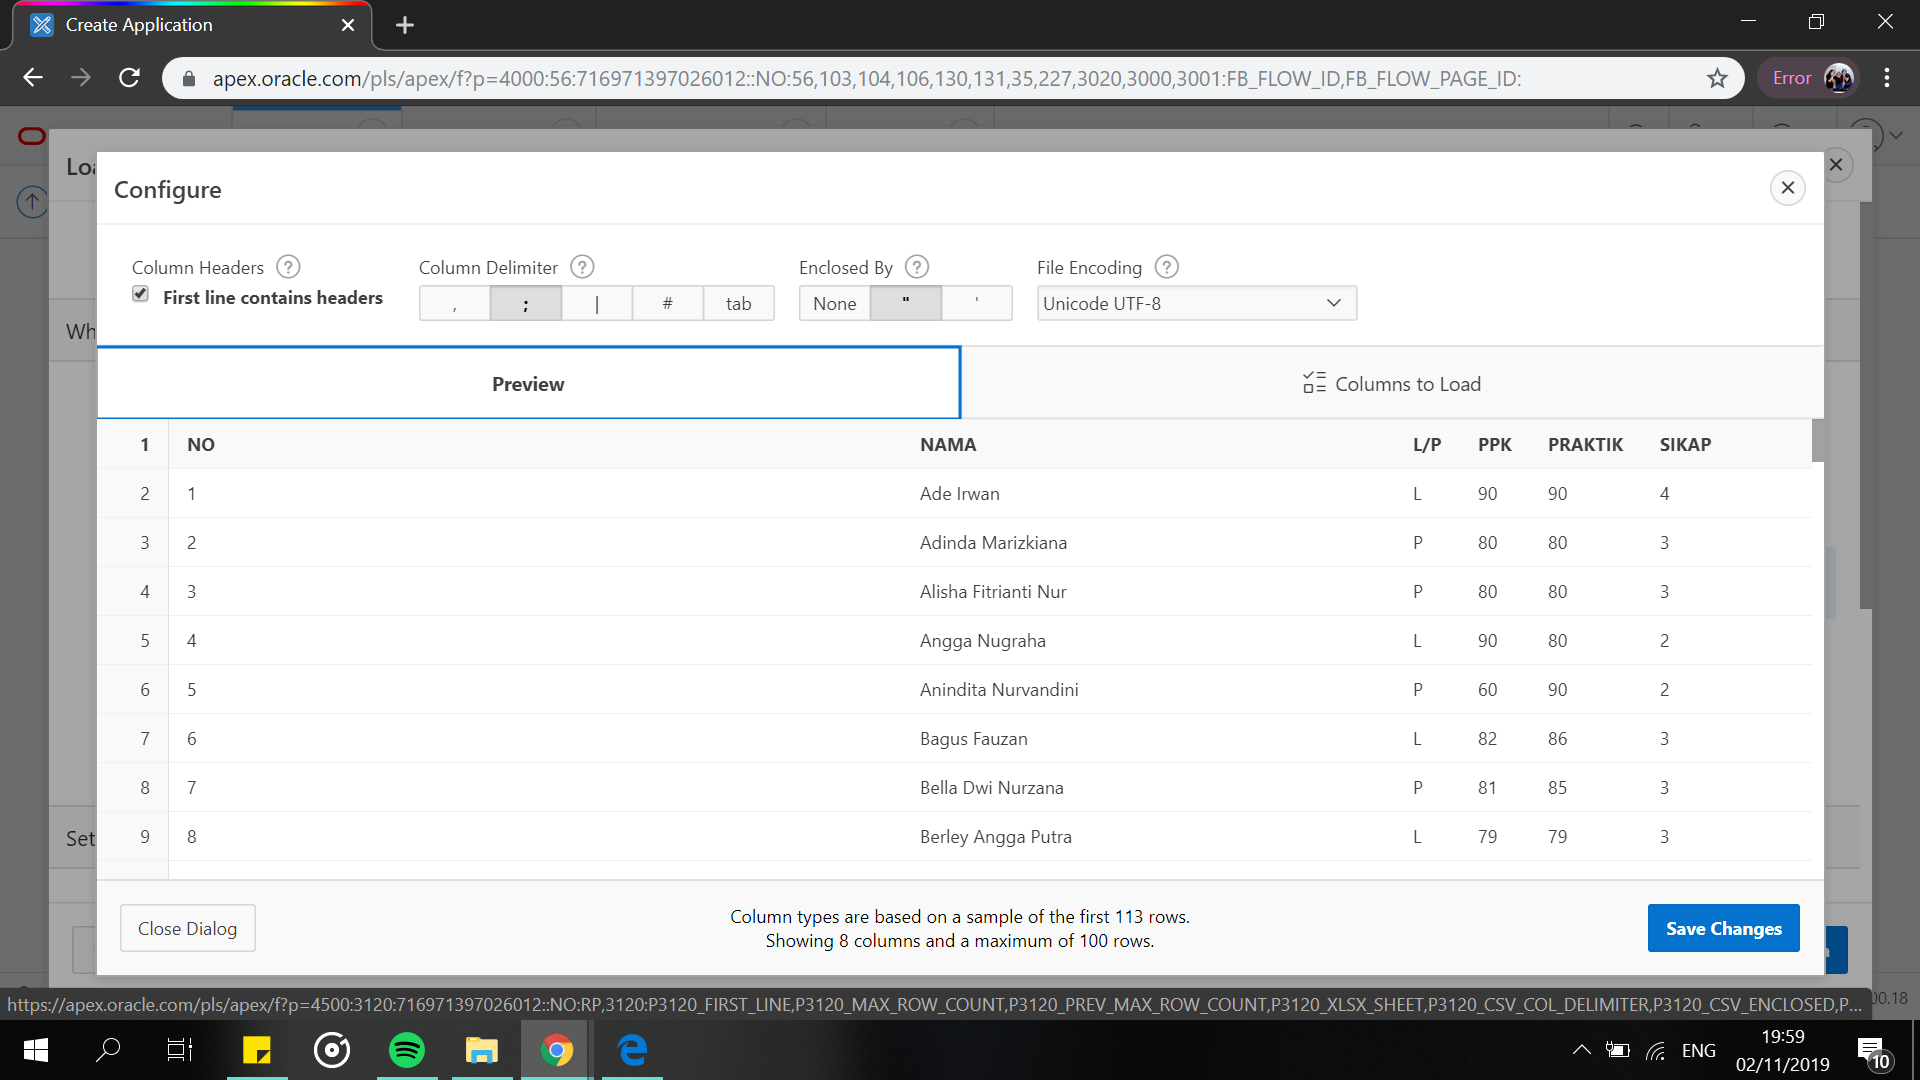
\includegraphics[width=9cm]{picture/05.png}
    \caption{Mengisi Nama Tabel}
    \end{figure}
    
    \begin{figure}[!htbp]
    \centering
    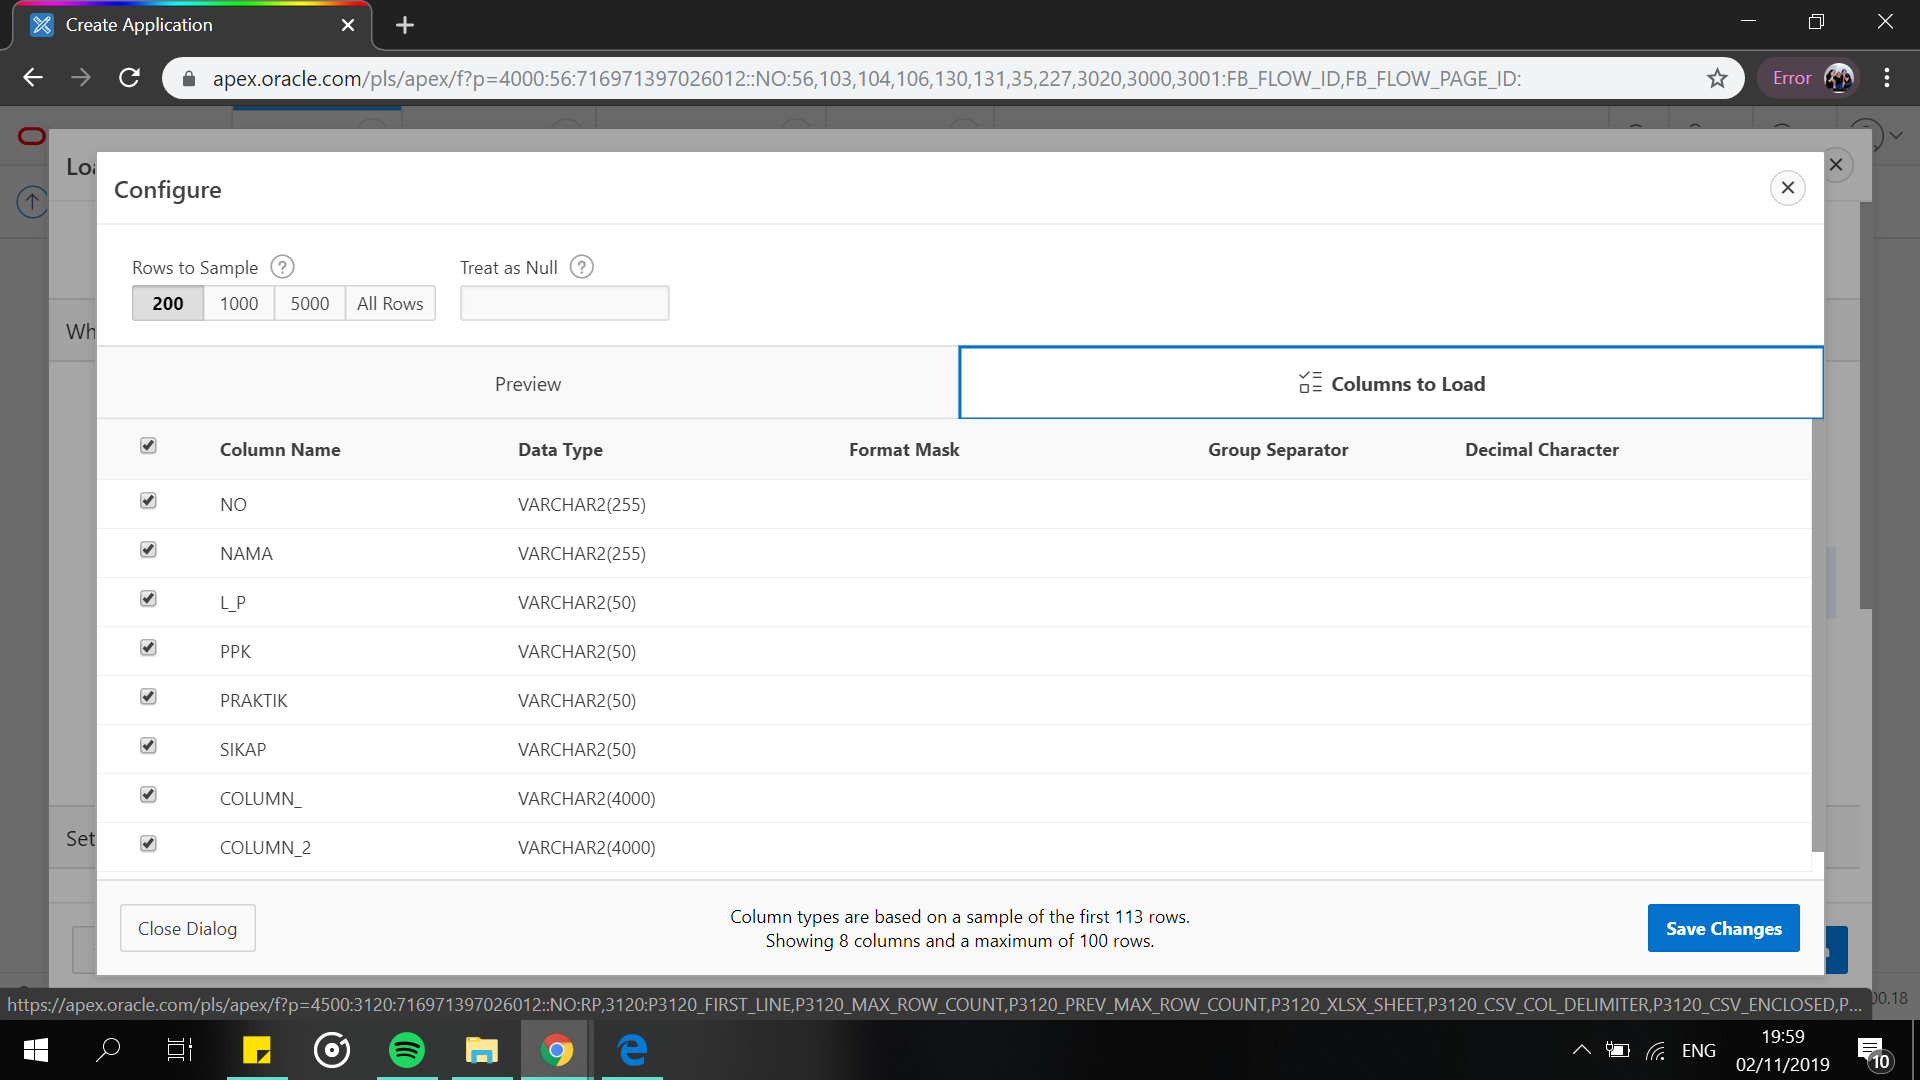
\includegraphics[width=9cm]{picture/06.png}
    \caption{Mengisi Nama Tabel}
    \end{figure}
    
    \begin{figure}[!htbp]
    \centering
    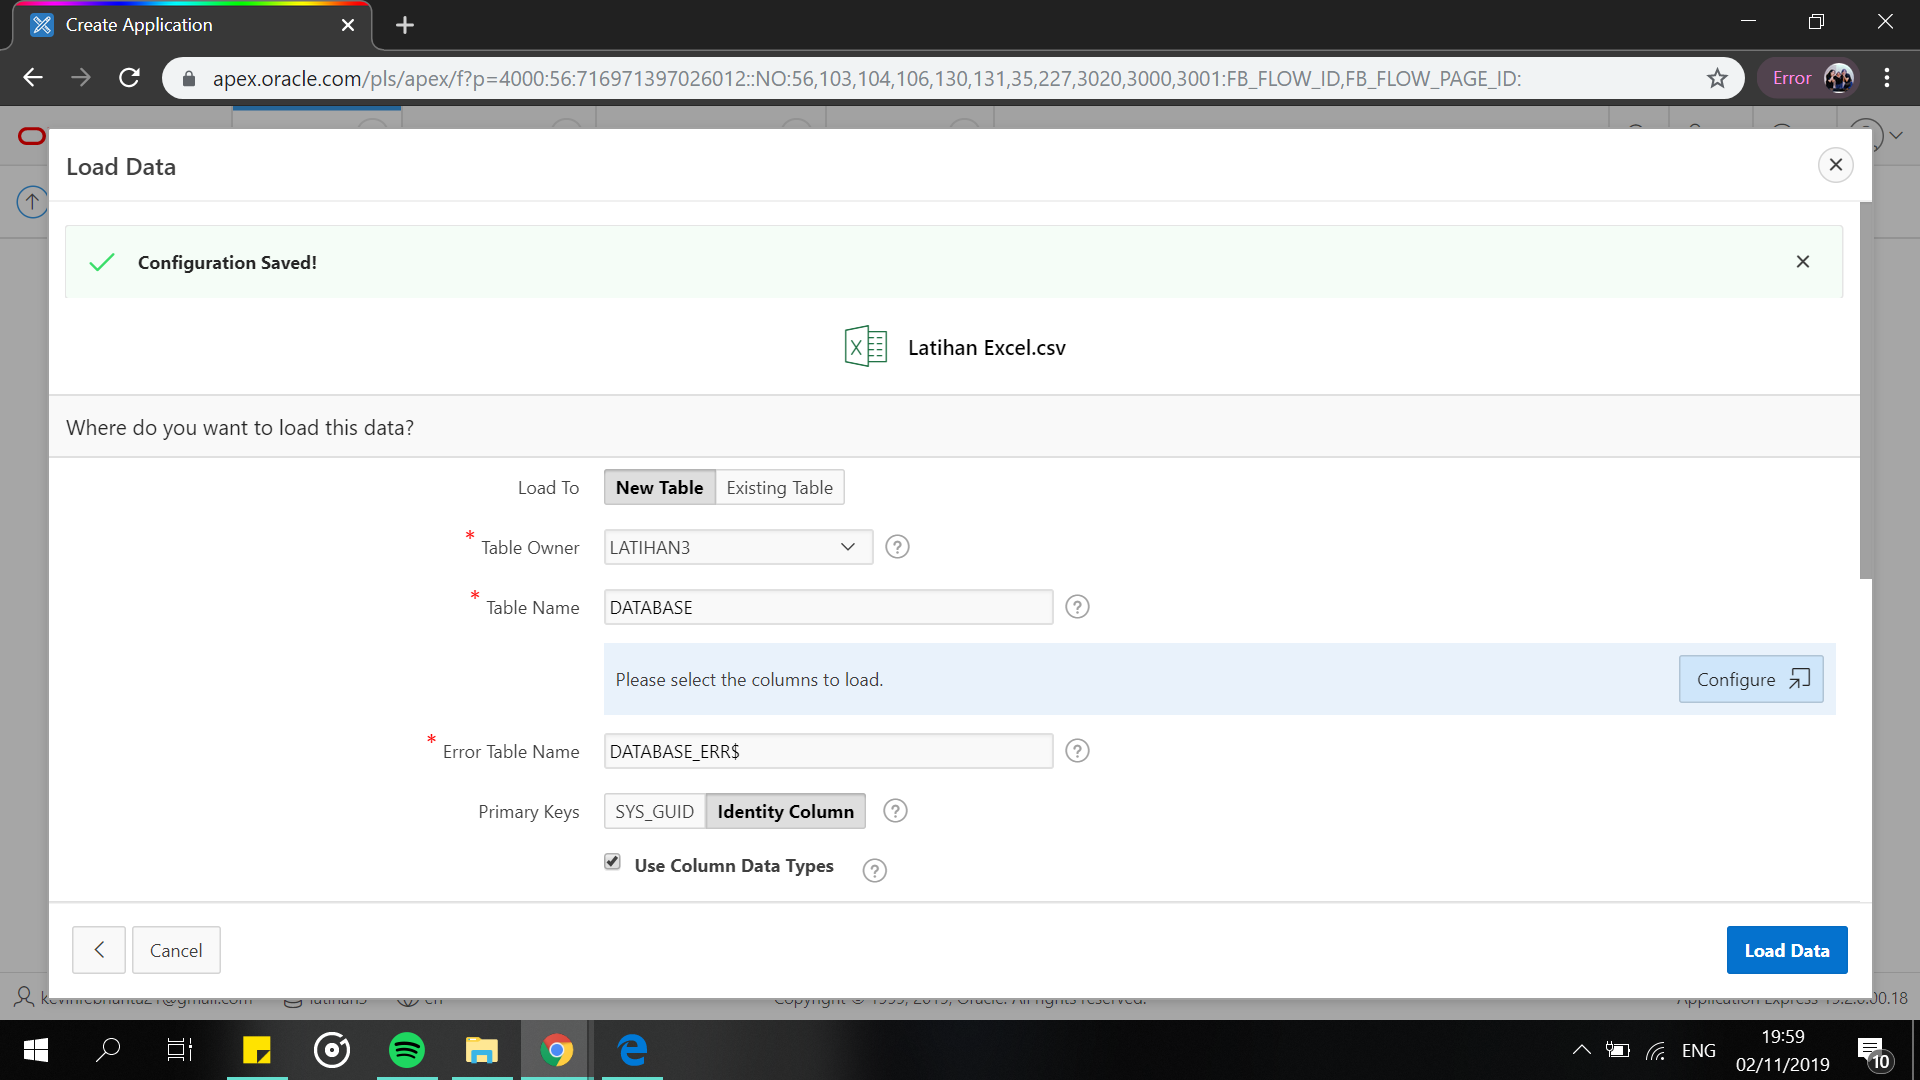
\includegraphics[width=9cm]{picture/07.png}
    \caption{Mengisi Nama Tabel}
    \end{figure}
    
\newpage
\item Kita pilih save changes..untuk menyipan data yang telah diinput
    \begin{figure}[!htbp]
    \centering
    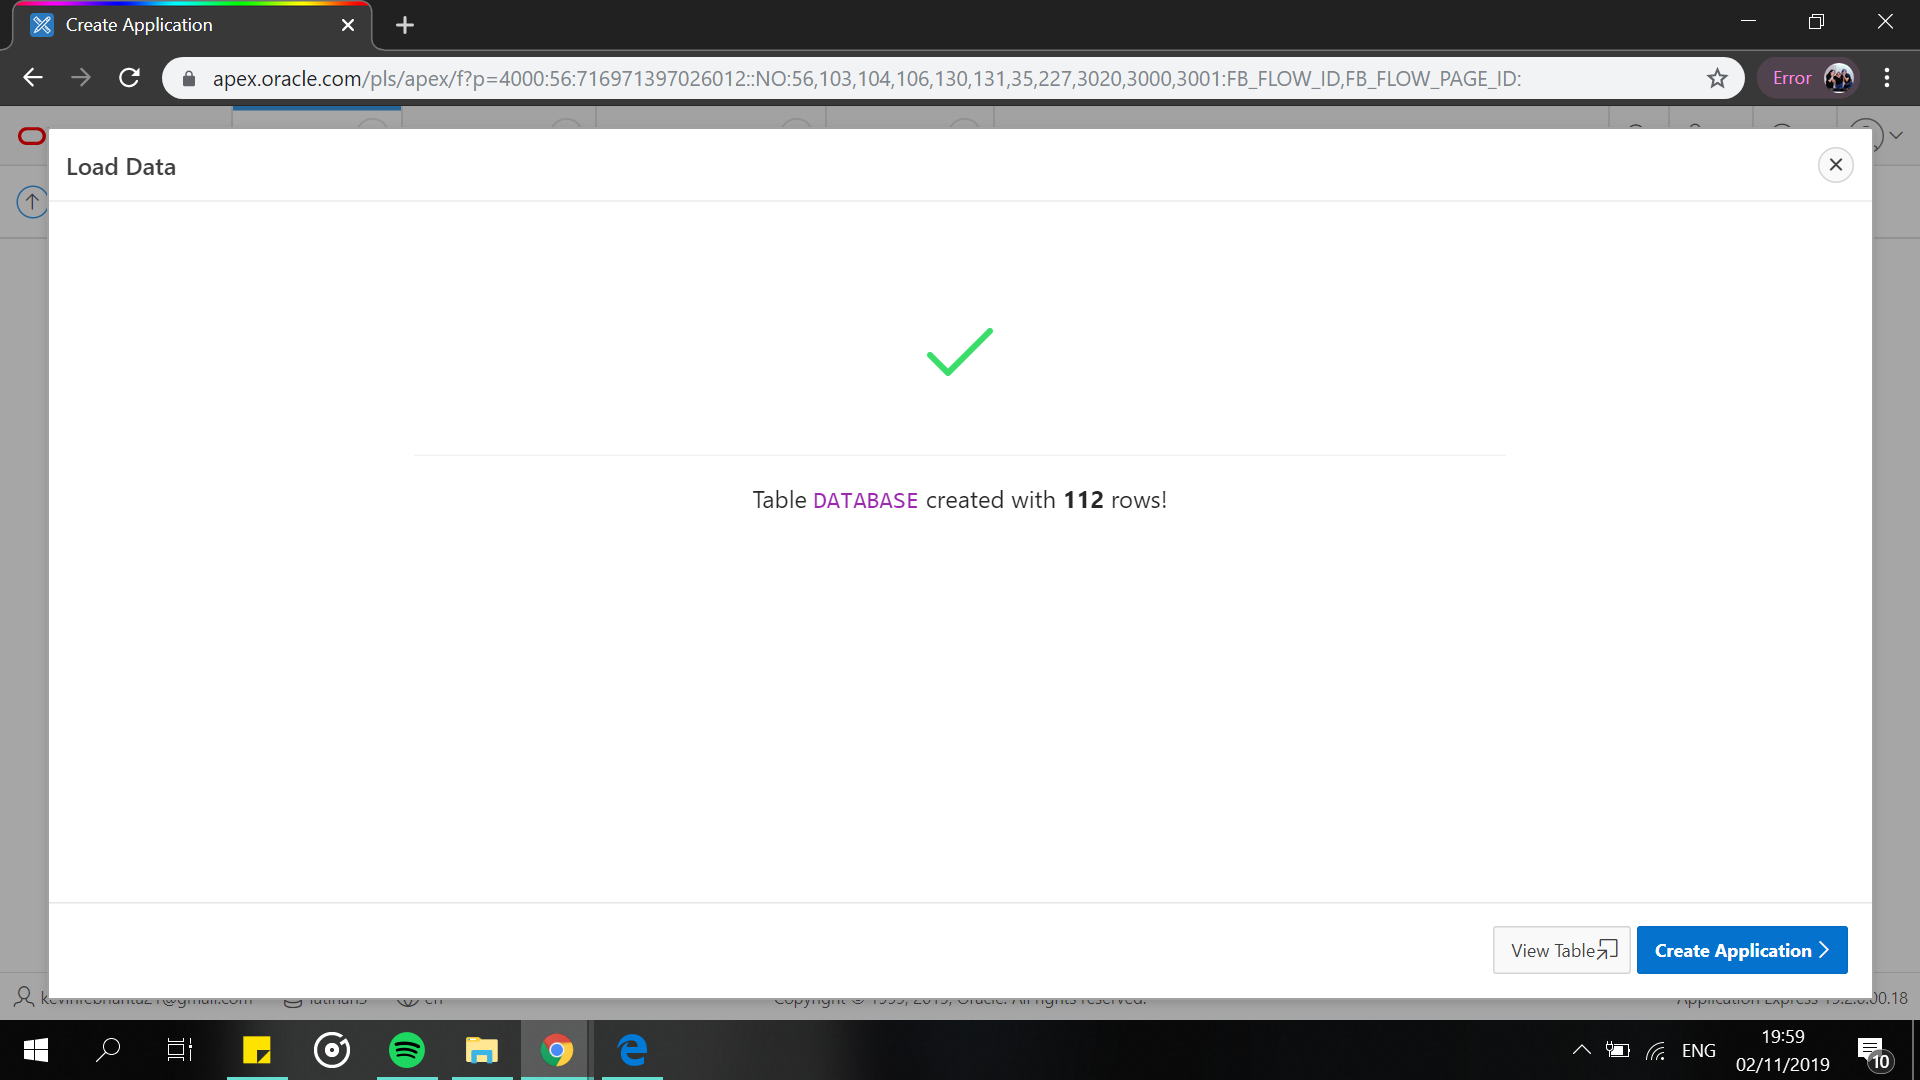
\includegraphics[width=9cm]{picture/08.png}
    \caption{Save Tabel}
    \end{figure}
    
\item Selanjutnya kita pilih create apllication,jika sudah tampil seperti ini
    \begin{figure}[!htbp]
    \centering
    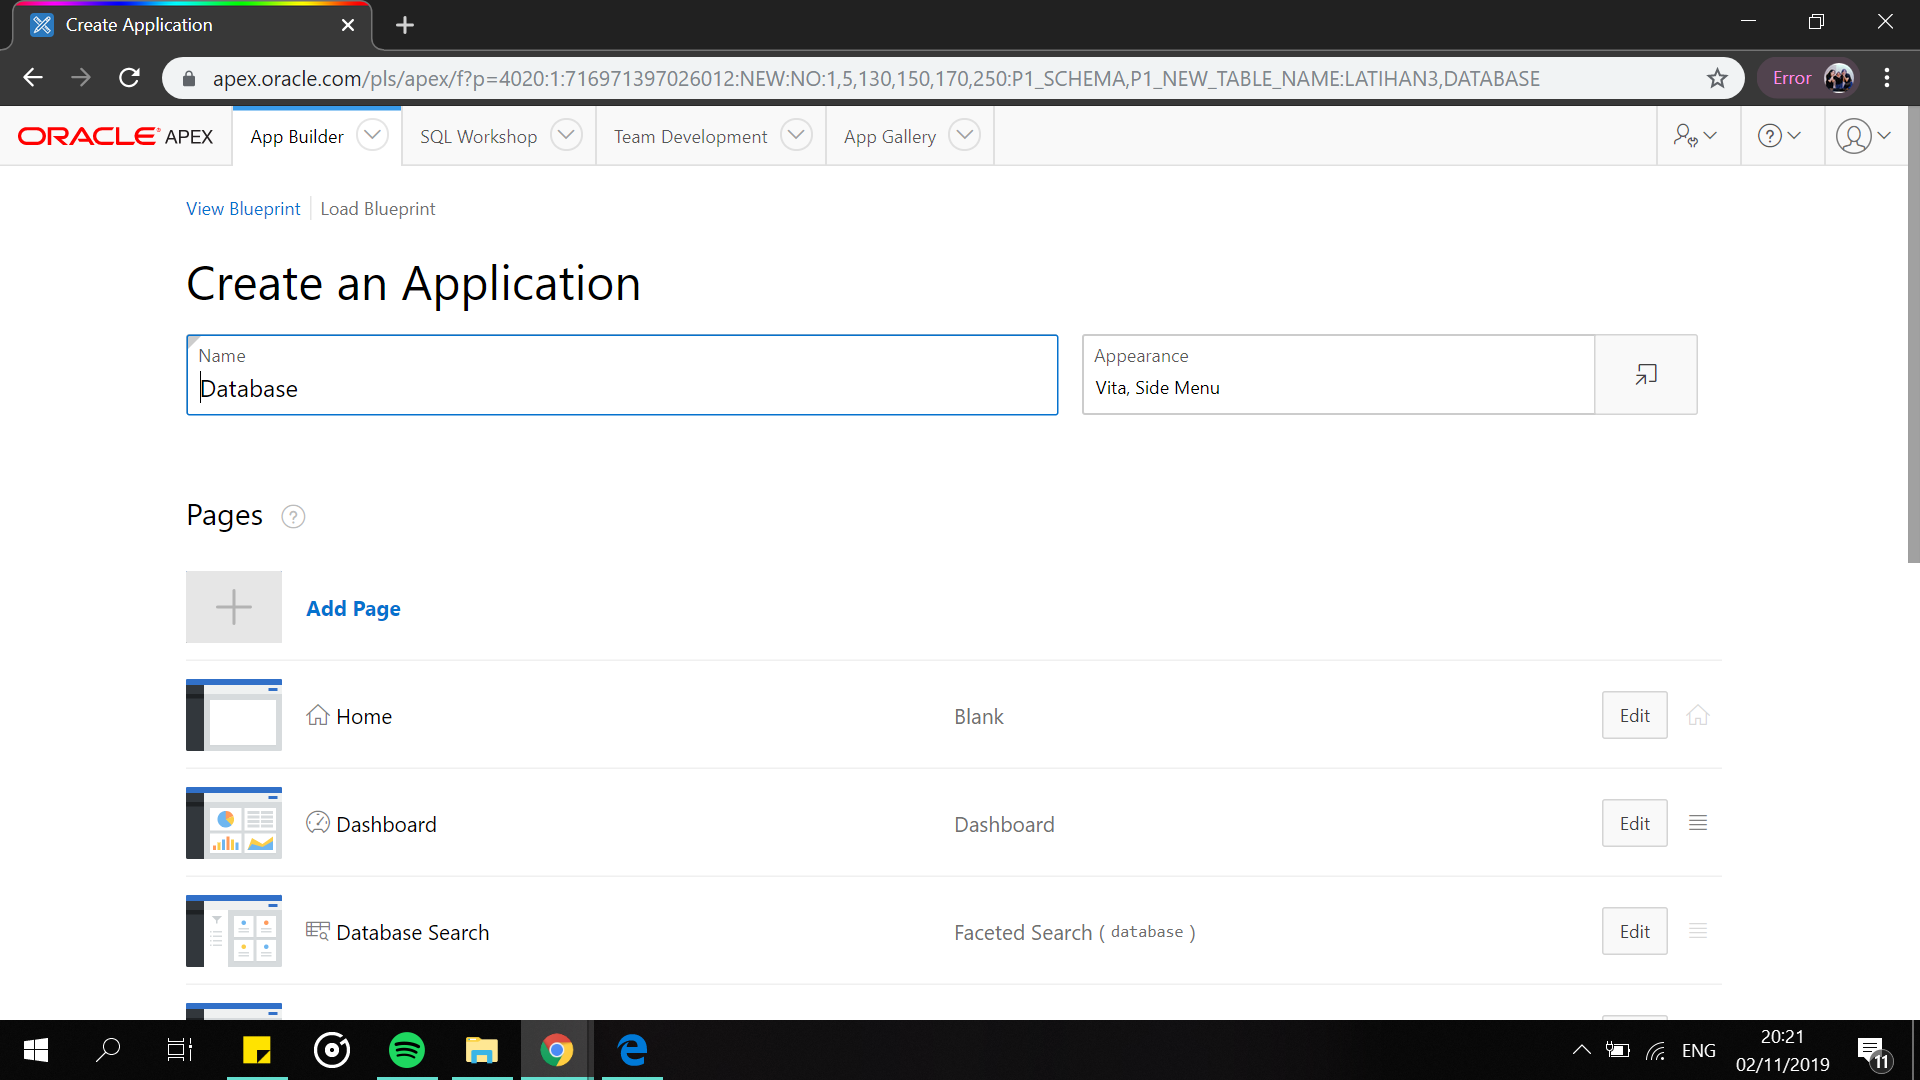
\includegraphics[width=9cm]{picture/10.png}
    \caption{Create Application}
    \end{figure}

\item  Create Application
    \begin{figure}[!htbp]
    \centering
    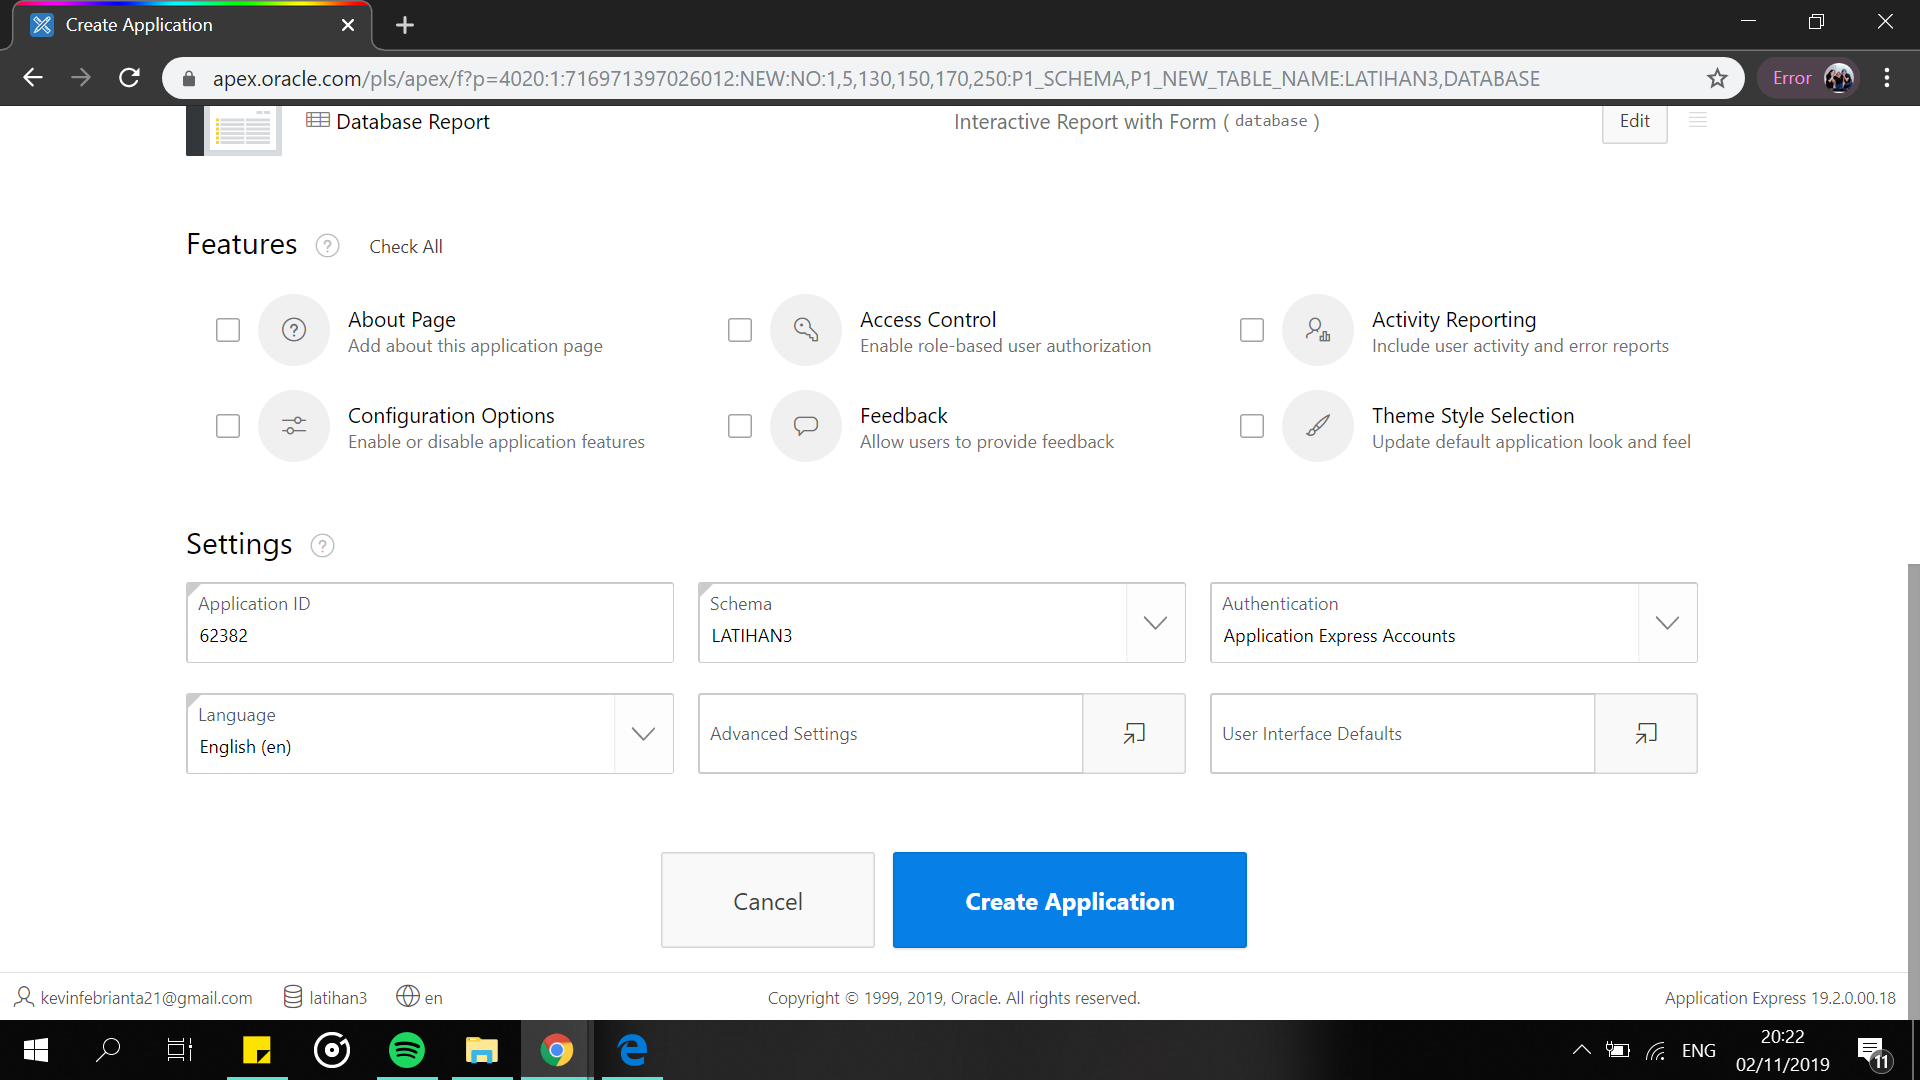
\includegraphics[width=9cm]{picture/11.png}
    \caption{Create Application}
    \end{figure}

\newpage    
    \begin{figure}[!htbp]
    \centering
    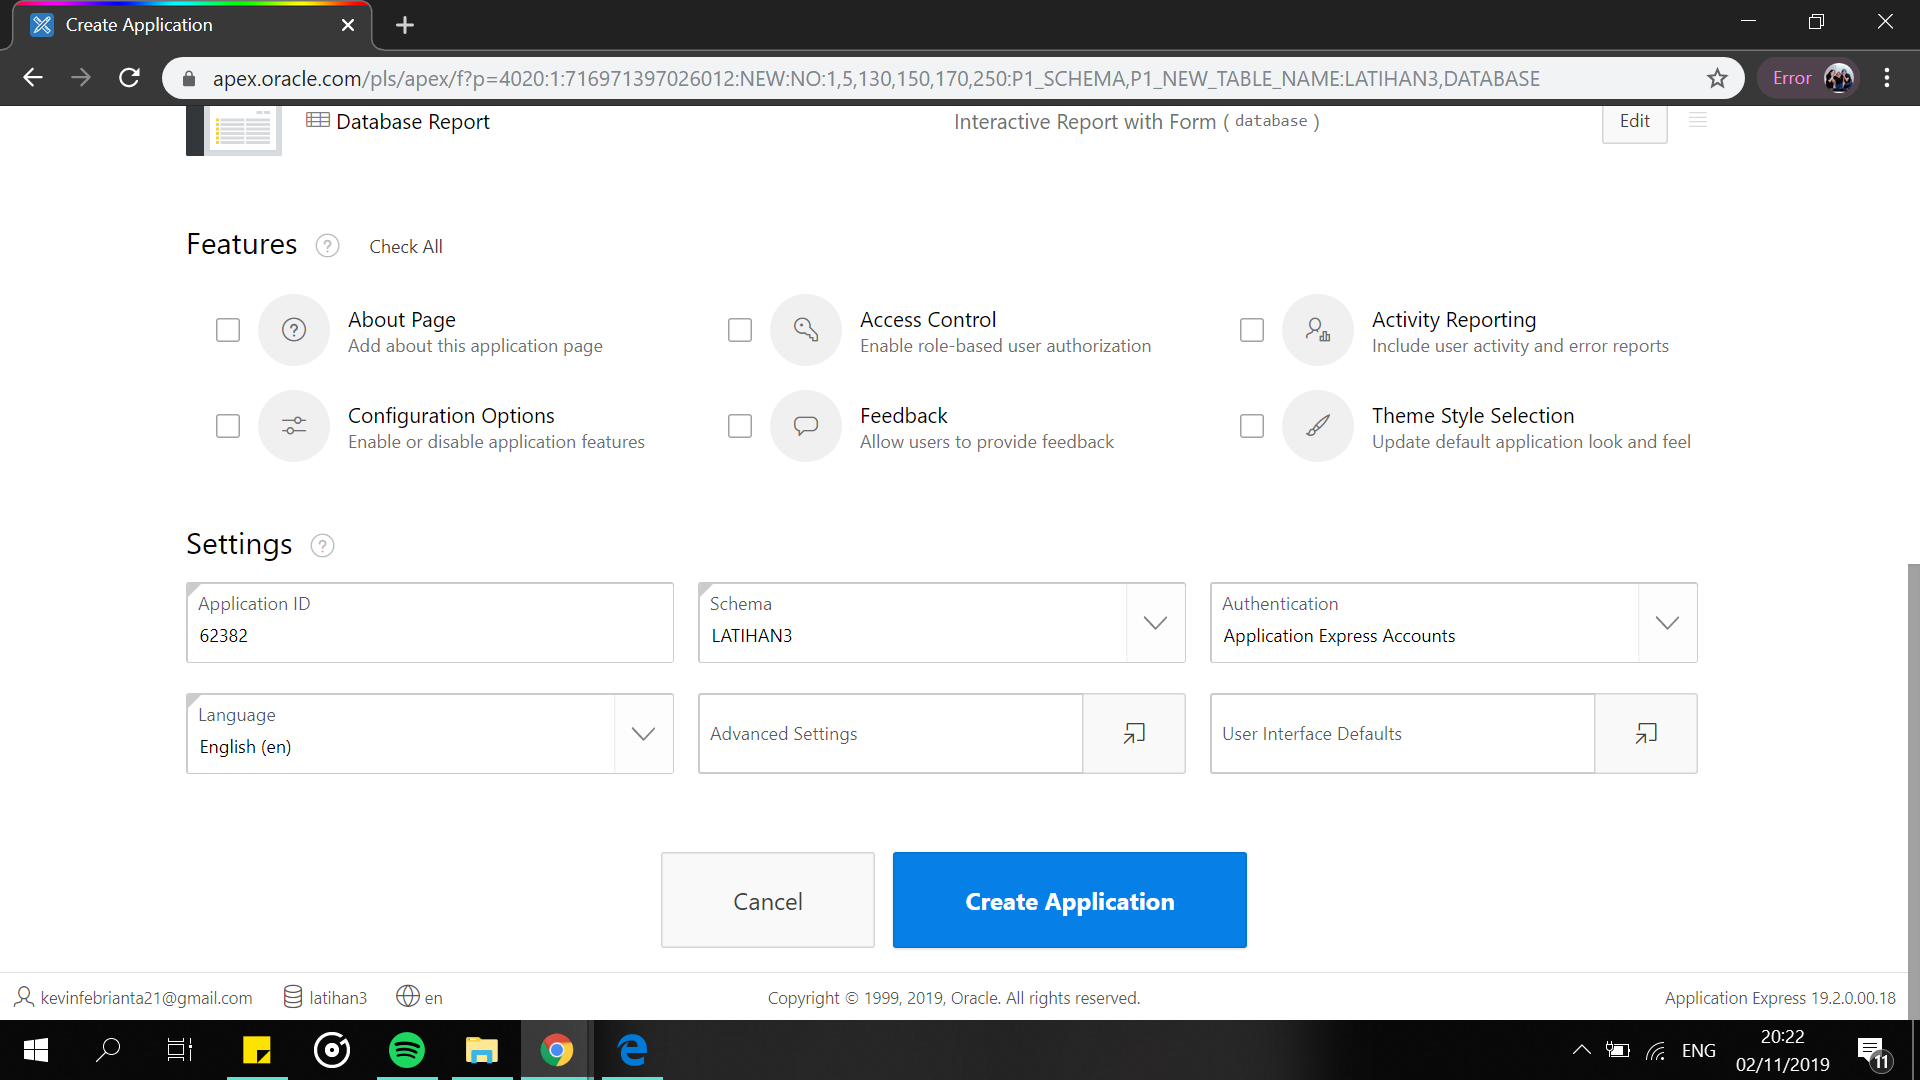
\includegraphics[width=9cm]{picture/11.png}
    \caption{Create Application}
    \end{figure}
        
\item Run Application
    \begin{figure}[!htbp]
    \centering
    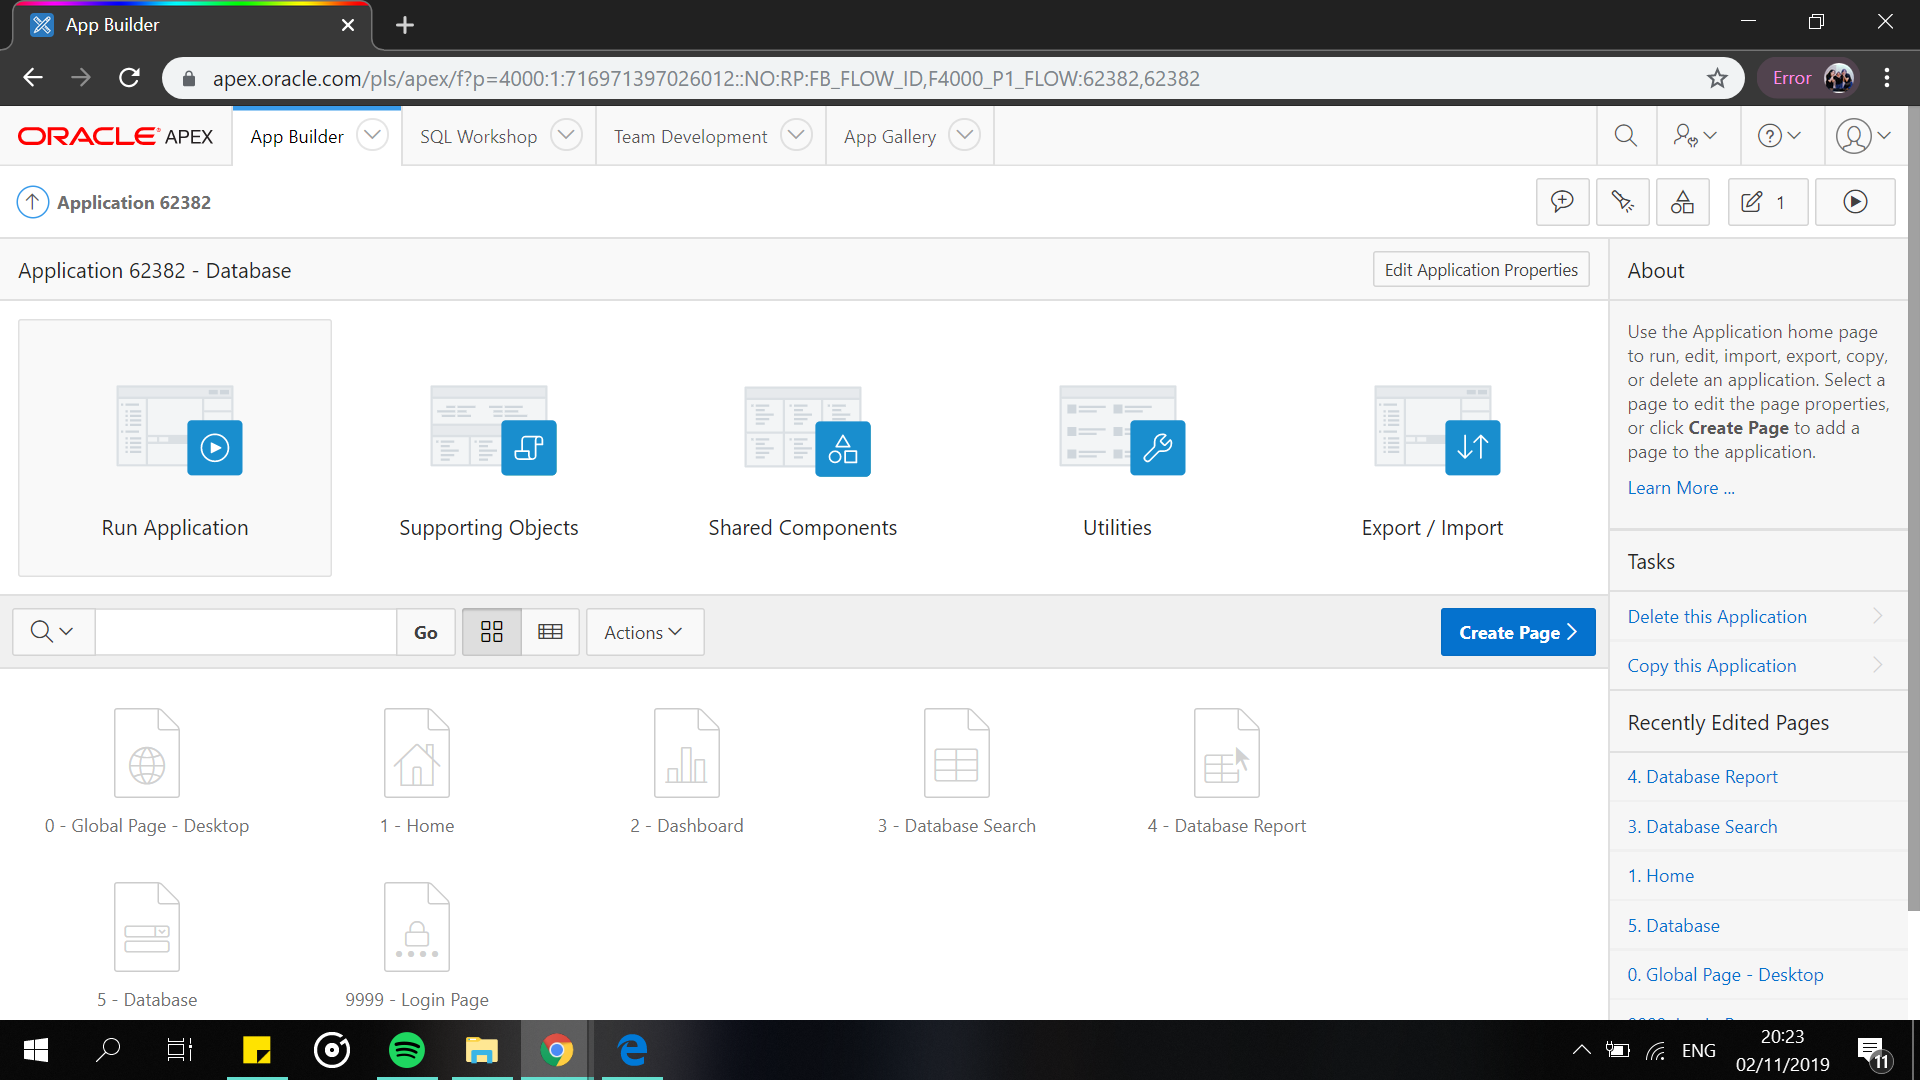
\includegraphics[width=9cm]{picture/12.png}
    \caption{Run Application}
    \end{figure}
    
\item Sign In akun oracle.
    \begin{figure}[!htbp]
    \centering
    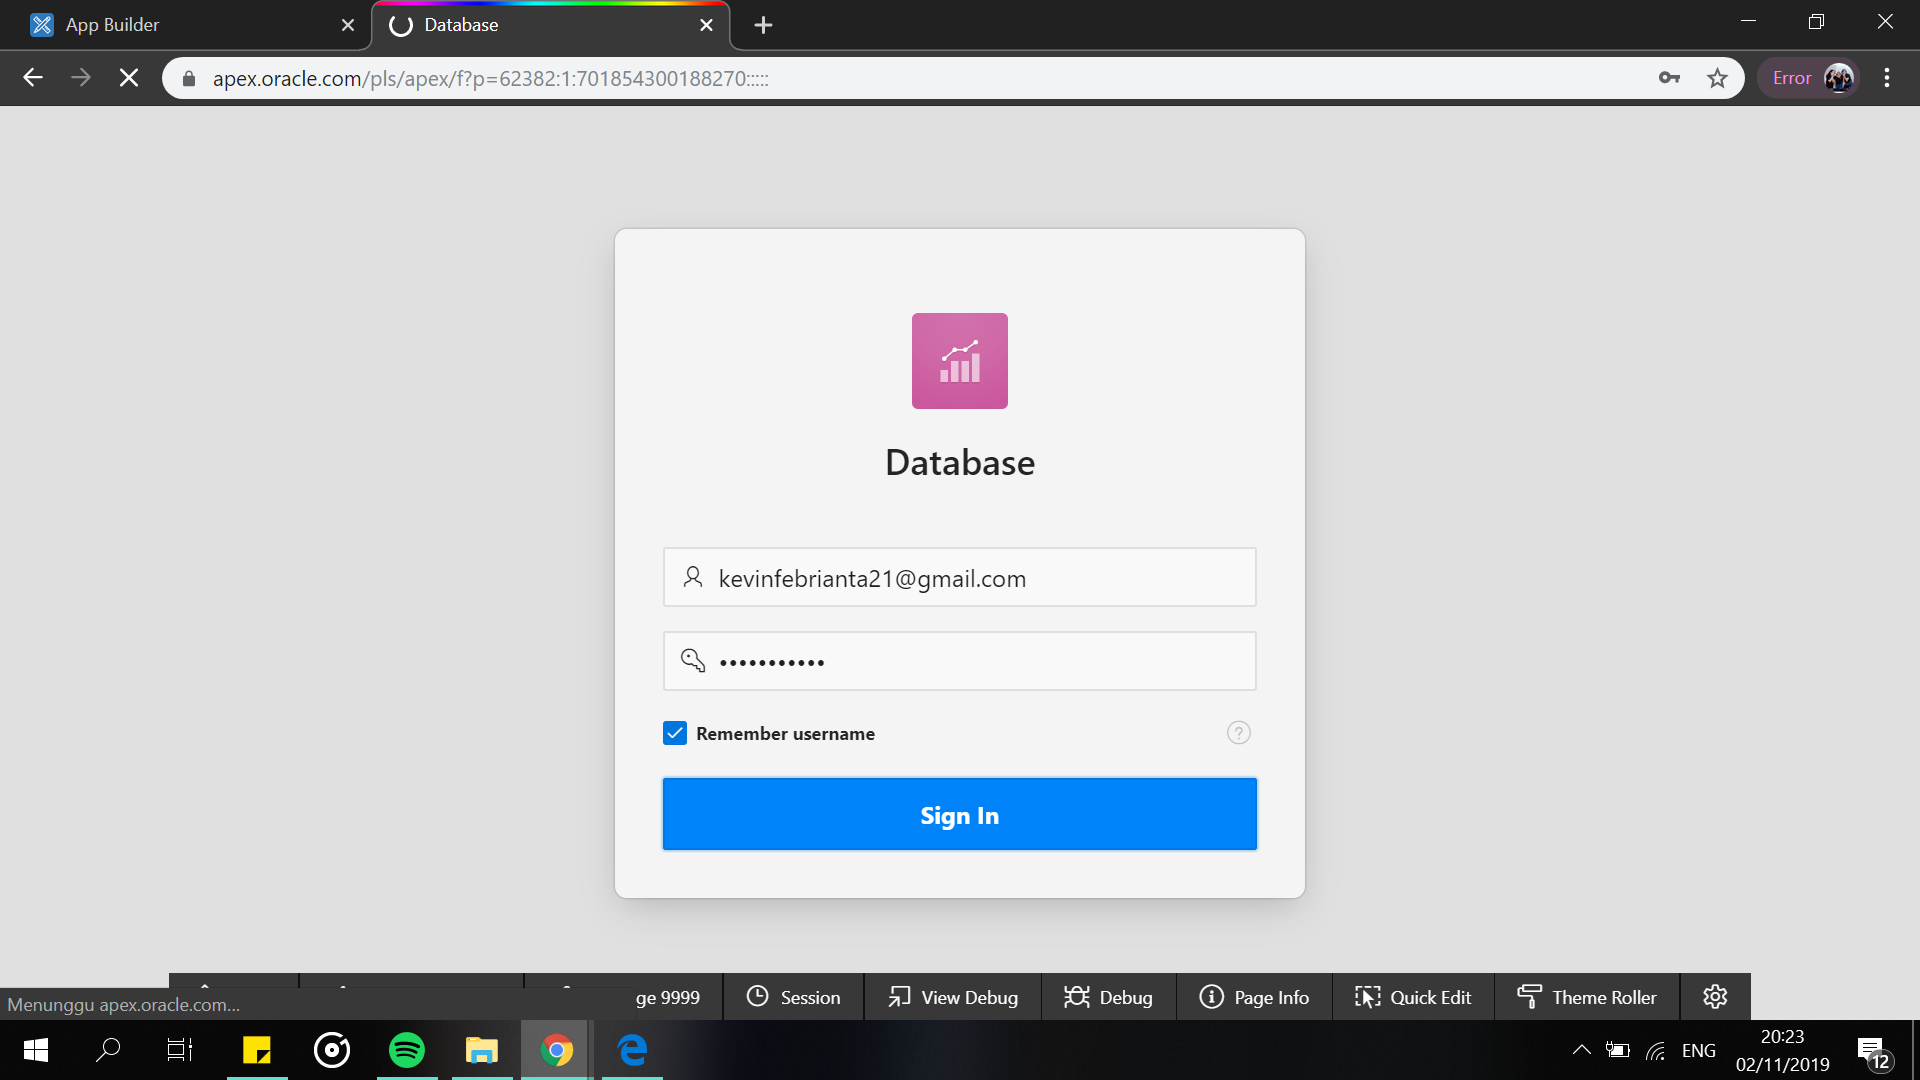
\includegraphics[width=9cm]{picture/13.png}
    \caption{Sign In Oracle}
    \end{figure}
    
\newpage
\item Telah berhasil masuk
    \begin{figure}[!htbp]
    \centering
    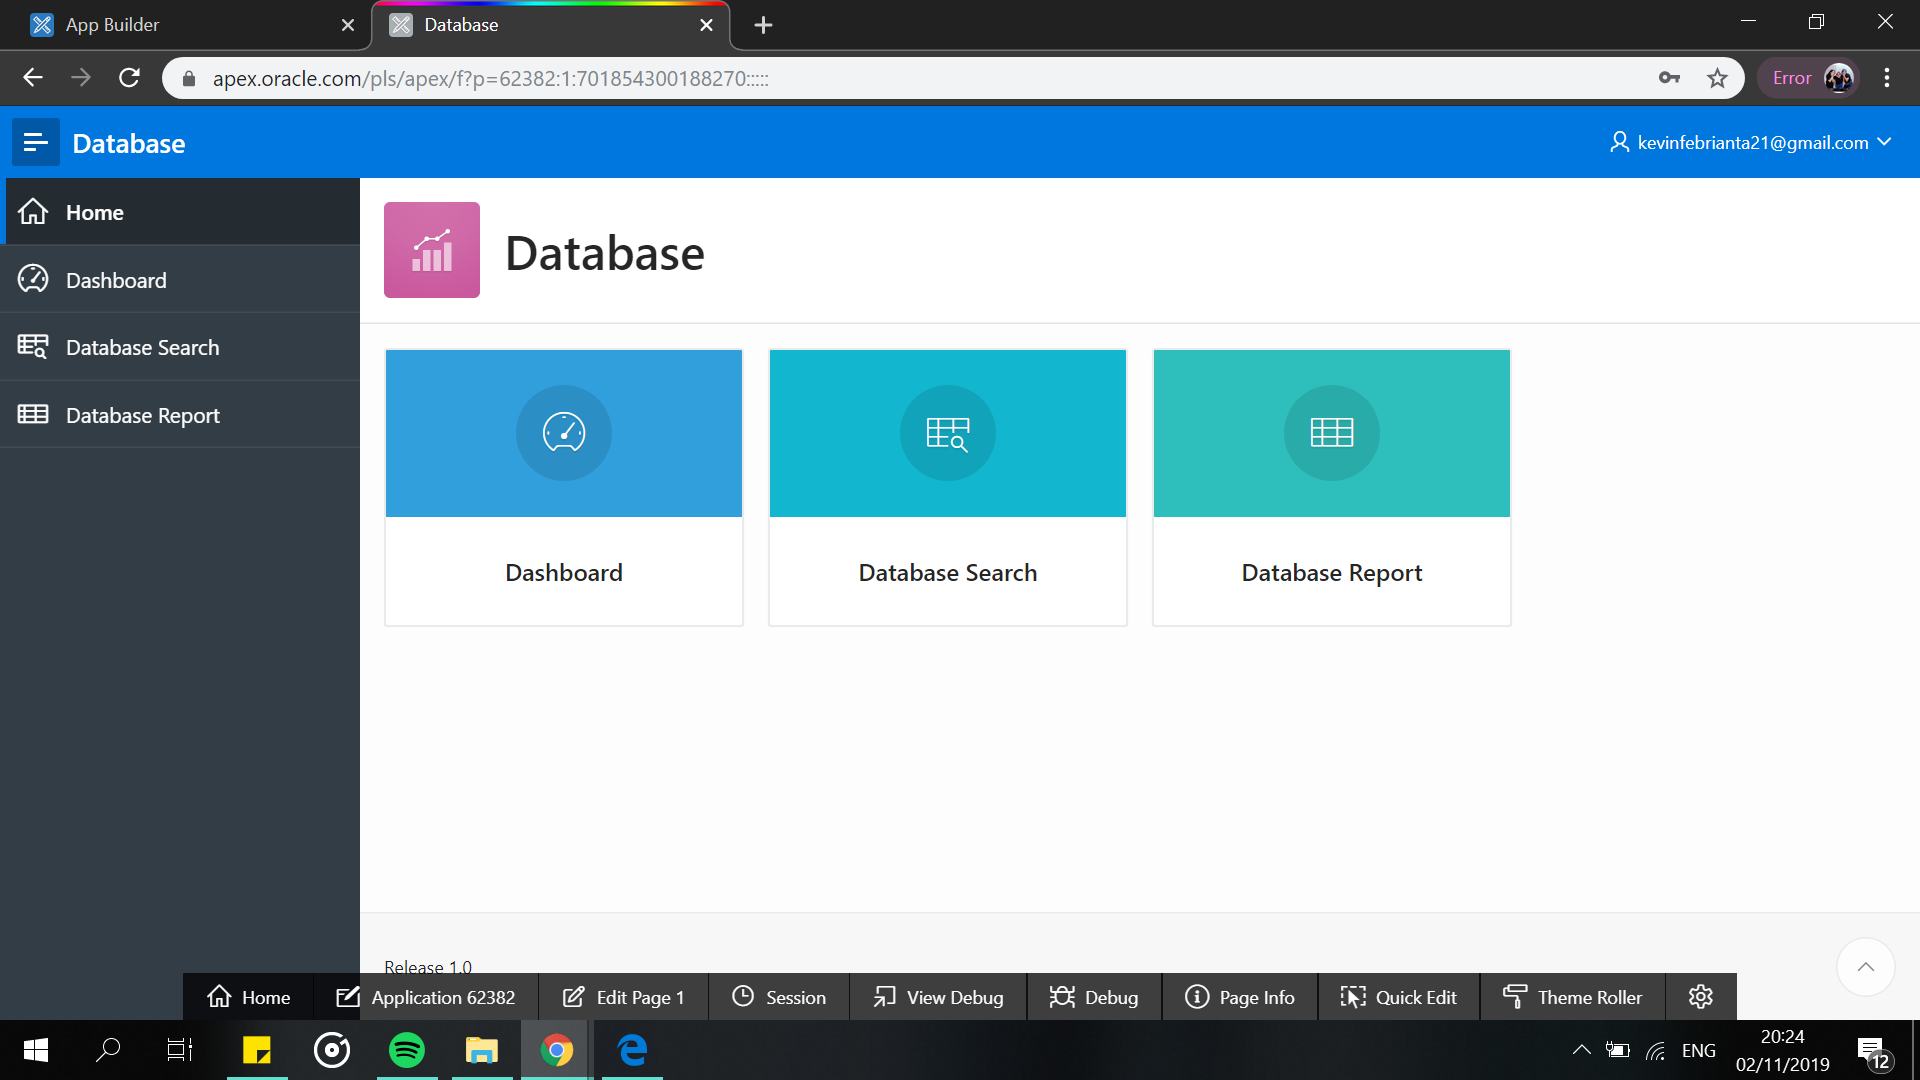
\includegraphics[width=9cm]{picture/14.png}
    \caption{Application}
    \end{figure}

    
    
\end{enumerate}